
%  $Description: Author guidelines and sample document in LaTeX 2.09$  $Author:
% ienne $ $Date: 1995/09/15 15:20:59 $ $Revision: 1.4 $

\documentclass[times, 11pt,twocolumn]{article}
\usepackage{latex8}
\usepackage{times}
\usepackage{graphicx}
\usepackage{listings}
\usepackage{epsfig}



% ------------------------------------------------------------------------- take
% the % away on next line to produce the final camera-ready version
\pagestyle{empty}

% -------------------------------------------------------------------------
\begin{document}
\lstset{language=Haskell, numbers=left,
numberstyle=\tiny,numbersep=5pt,basicstyle=\scriptsize,aboveskip=10pt}

\title{Towards a Crosscutting Approach for Variability Management}

\author{Rodrigo Bonif\'{a}cio and Paulo Borba\\
Informatics Center \\ Federal University of Pernambuco \\ Recife, Brazil \\
\{rba2, phmb\}@cin.ufpe.br\\ }

\maketitle
\thispagestyle{empty}

\begin{abstract}
   The ABSTRACT is to be in fully-justified italicized text, at the top 
   of the left-hand column, below the author and affiliation 
   information. Use the word ``Abstract'' as the title, in 12-point 
   Times, boldface type, centered relative to the column, initially 
   capitalized. The abstract is to be in 10-point, single-spaced type. 
   The abstract may be up to 3 inches (7.62 cm) long. Leave two blank 
   lines after the Abstract, then begin the main text. 
\end{abstract}



%------------------------------------------------------------------------- 
\Section{Introduction}\label{sec:intro}

In order to reduce time-to-marketing and improve quality of software products,
several approaches and techniques for economy of scope, mass customization, and
systematic reuse have been recently proposed. Examples of such approaches include \emph{Software Product
Lines}~\cite{Pohl:2005aa, Clements:2001aa}, \emph{Generative Programming
Techniques}~\cite{Czarnecki:2000aa}, and \emph{Software
Factories}~\cite{Greenfield:2003aa}. Actually, there is a lot in common among
such approaches. For instance, one common characteristic is the relevance of
domain analysis, which aims at defining a scope (often in the business sense)
in which reusable assets can be used for generating specific products.

Additionally, it is a common practice to use \emph{feature modeling} for
representing features that are common to all products within a scope and which
features are optional, being useful for diferentiating specific products in a
family. Therefore, aiming to generate specific products, it would be necessary
to: (a) introduce suitable variation points in common assets, (b) develop
variant assets that extend these variation points, and (c) relate features to both common and
variant assets.

In this work, we consider \emph{variability management} as the discipline that
guides these activities. Actually, variability management is an interesting kind
of crosscutting concern, since certain features require variation points to be
spread in different places of requirements, design, code, and test artifacts.
This crosscutting nature of variability management results in interesting
challenges regarded to SPL traceability, evolvability, and product derivation. As
a consequence, several authors have proposed the use of \emph{aspect-oriented}
techniques to better modularize the composition of common and variant assets of a
product line~\cite{}. In this thesis we go beyond this composition issue. We
mainly consider a more encompassing notion of variability management, presenting
its semantics as a crosscutting concern and describing the contribution of
relevant artifacts (such as feature models and configuration knowledge) in
product generation.

Our hypotheses is that a clear separation between variability management and
common software engineering artifacts improves SPL evolvability, traceability,
and product derivation. A clear separation means that each SPL model (feature
model, configuration knowledge, SPL use case model, and so on) should focus on
specific concerns. For instance, use case models should represent just the valid
interactions with a software. They should not be enriched to describe variability
space (as proposed in~\cite{Bertolino:2003aa}). The challenge is that, in order
to generate specific products, the clear separation that we are proposing
requires composition processes involving different SPL models. In this thesis,
we define the semantics of composition processes as crosscutting mechanisms.
The elegant notion of crosscutting mechanisms, formalized by Masuhara and
Kiczales~\cite{Masuhara:2003aa}, is used as underlining support for presenting
the semantics of our composition processes. 

Initial results of our approach, applied in the context of representing SPL
variabilities in use case scenarios, revealed to us improvements in both
evolvability and product generation~\cite{Bonifacio:2008aa}. The choice of applying our
approach in this context was motivated because current techniques for scenario variability
management~\cite{Eriksson:2005aa, Bertolino:2003aa} do not present a clear
separation between variability management and scenario specification.
In summary, the contributions of this thesis are threefold

\begin{itemize}
 \item Characterize the broader notation of variability management as
a crosscutting concern and, in this way, propose an approach for
representing it as an independent view of the SPL. Although
this work focuses on requirements artifacts, more specifically
use case scenarios, we argue that such separation is also required
in other SPL models.
 \item A framework for modeling the composition processes of scenario
variability mechanisms. This framework gives a basis for
describing variability mechanisms (such as scenario composition
and parameterization), allowing a better understanding of each mechanism and
highlighting the contribution of each model used in the composition processes.
In this work, such a framework is used for modeling the semantics of scenario variability mechanisms, but it
might be customized for other SPL views.
 \item A deeper evaluation of existing techniques for representing scenario
 variability. Such an evaluation will take into consideration not only the
 support for different variability techniques (parameterization, optional
 scenarios), but also a comparison of existing works with regard to
 SPL evolvability and traceability.  
\end{itemize}

The next section describes our approach, named as \emph{variability management
as crosscutting} (Section~\ref{sec:vmcc}). It also relates some open questions
of our approach, which we are going to solve in this thesis. After that,
Section~\ref{sec:evaluation} presents the results of three empirical studies,
which we have compared our proposed approach with existing
works. These comparisons were based on \emph{Design Structure Matrices} and on a
suite of metrics, addapted from aspect-oriented communit, for quantifying modularity.
We also present in Section~\ref{sec:evaluation} a discussion about several
improvements on our evaluation processes. Then, we relate our
thesis with existing works (Section~\ref{sec:related}) and present final concludings 
in Section~\ref{sec:concludings}.

%-------------------------------------------------------------------------
\section{Variability management as crosscutting}\label{sec:vmcc}

As we said in the previous section, we are proposing an approach for
variability management that aims to separate variability models
from common software engineering models. However, once these concerns 
had been saparated, it would be necessary to weave those models in order to 
generate specific products. Moreover, in this work we consider variability
management as a crosscutting concern, since certain features require variation
points to be spread in different places of SPL artifacts. 

In order to represent variability management as a crosscutting concern, we
proposed a modeling framework (Section~\ref{sub:framework}), that slightly
generalizes the Masuhara and Kiczales (MK) framework~\cite{Masuhara:2003aa}, and instantiate it for the 
product line domain. The MK framework aims to explain
how different \emph{aspect-oriented} technologies support crosscutting
modularity. In their proposed approach, each technology is modeled as a
three-part description: the related weaving processes take two programs as input, 
which crosscut each other with respect to the resulting program or
computation~\cite{Masuhara:2003aa}.

Specifically in the context of use case scenario variabilities, we represent the
semantics of \textbf{scenario variability management} as a weaver that takes as input four specifications
(\emph{product line use case model}, \emph{feature model}, \emph{product
configuration}, and \emph{configuration knowledge}) that crosscut each other with
respect to the resulting product specific use case model
(Figure~\ref{fig:weave-process}). Combining these input languages, it is possible
to represent the kinds of variability that we are interested in: \emph{optional
use cases and scenarios}, \emph{quantified changed scenarios}, and
\emph{parameterized} scenarios.

\begin{figure}[t]
 \begin{center}
  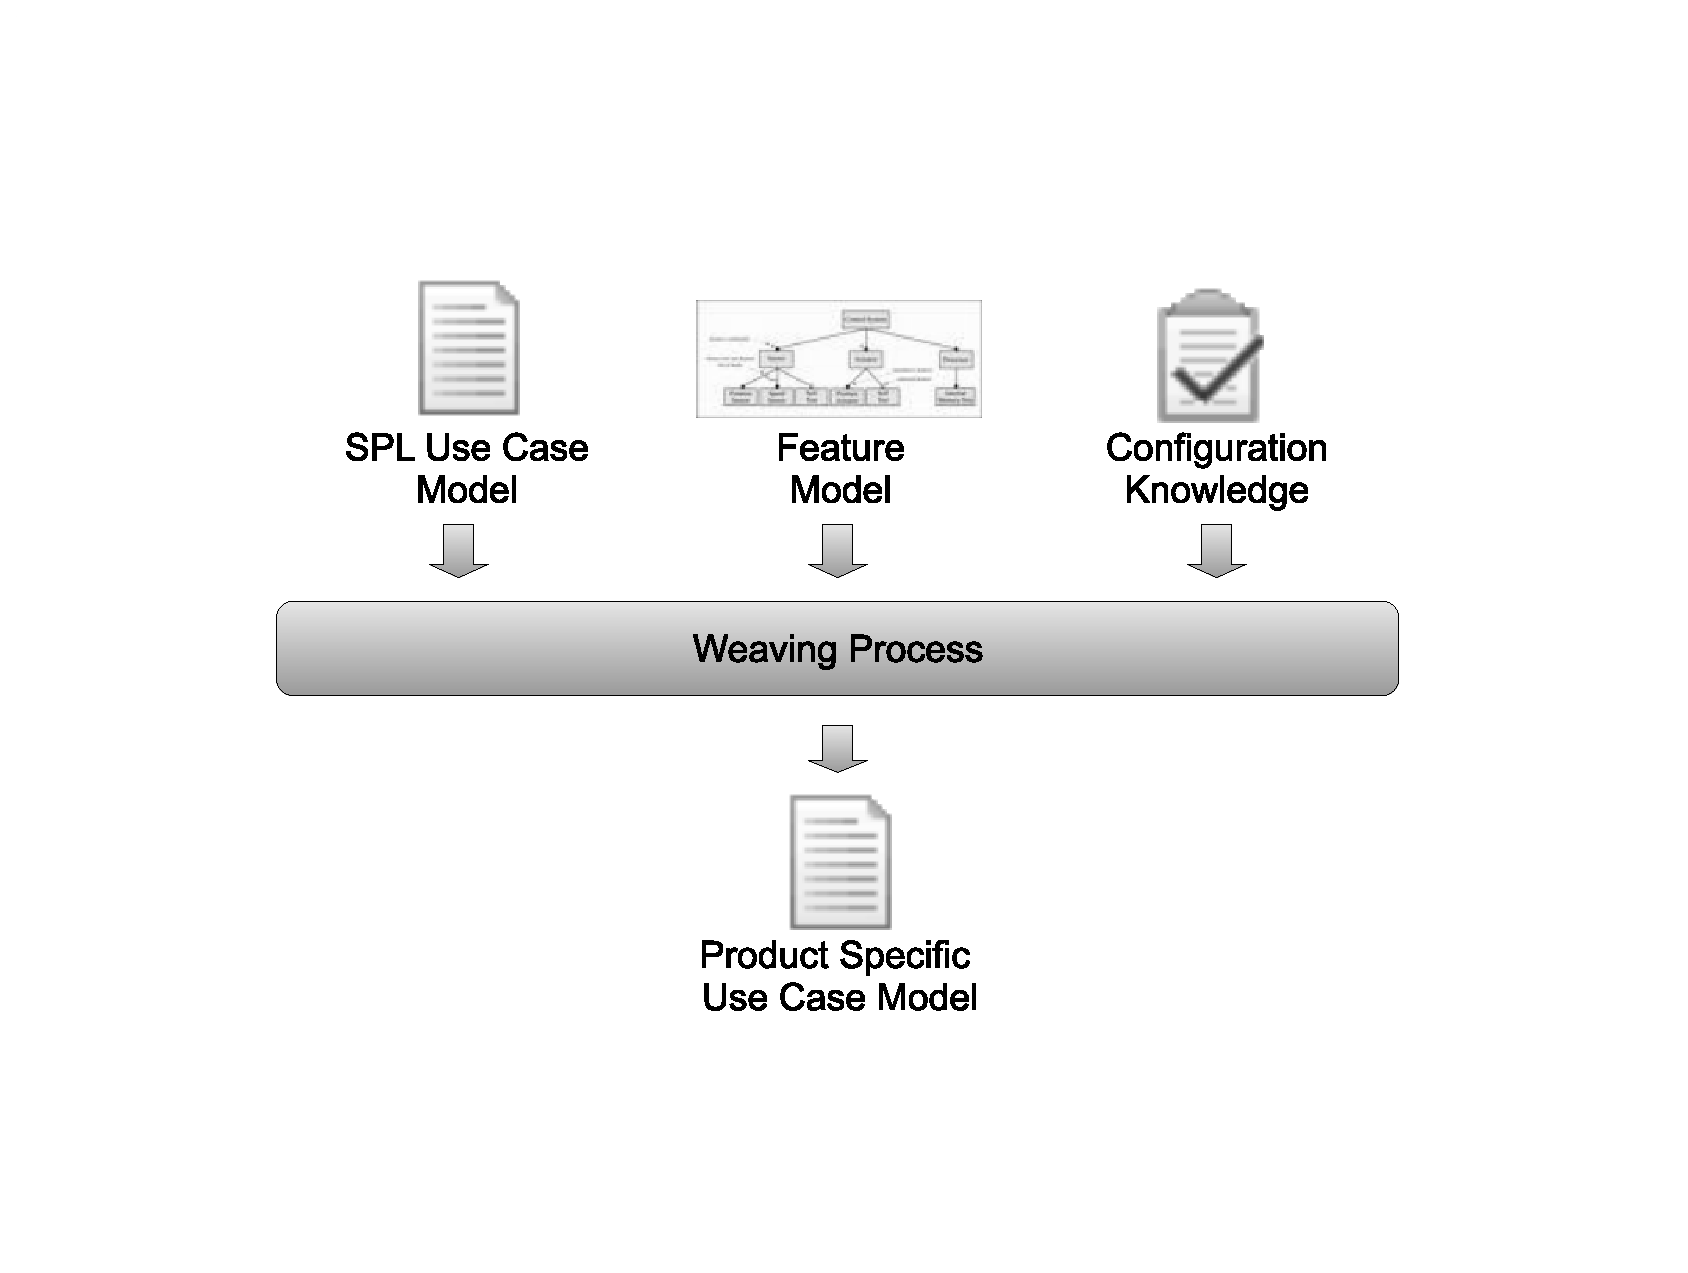
\includegraphics[scale=0.35]{../images/weave-process.eps}
  \caption{Overview of our weaving process.}
  \label{fig:weave-process}
  \end{center}
\end{figure}

In what follows, we present our modeling framework, proposed to explain
variability management as a crosscutting concern. Then, we instantiate such a
framework (Section~\ref{sub:framework-instance}) for representing one scenario
variability technique --- optional use cases and scenarios. More details about our approach can be found
elsewhere~\cite{}.

\subsection{Modeling framework}\label{sub:framework}

As explained before, our modeling framework, proposed for representing 
variability management weaving processes, is based on the Masuhara and Kiczales
work~\cite{Masuhara:2003aa}. Thereby, we describe each variability technique
as a weaver. In our work, we represent these weavers as an
\emph{6-tuple} (see Eq.~\ref{eq:tuple} and Table~\ref{tab:tup-01}), in
such a way that we can describe the contribution of each input model used 
in the composition process (Figure~\ref{fig:weave-process}).

\begin{equation}
Weaver = \{o, o_{jp}, L, L_{id}, L_{eff}, L_{mod}\}, 
\label{eq:tuple}
\end{equation}

\begin{table}[bth]
\begin{center}
\caption{Modeling framework elements.} \label{tab:tup-01}
\begin{tabular}{|p{0.6in}|p{2.4in}|}
  \hline
  {\bf Element} & {\bf Description} \\ 
   \hline
  $o$          & Output language used for describing the results of the weaving process \\ \hline
  $o_{jp}$     & Set of join points in the output language \\ \hline
  $L$          & Set of languages used for describing the input specifications \\ \hline
  $L_{ID}(l)$  & Set of constructions in each input language $l$, used for identifying the output join points \\ \hline 
  $L_{EFF}(l)$ & For each input language $l$, this element represent the effect of its constructions in the weaving process \\ \hline
  $L_{MOD}(l)$ & Set of modular unities of each input language $l$\\ \hline
  \hline
\end{tabular}
\end{center}
\end{table}

As a consequence, we model each variation technique by filling in
the six parameters of our \emph{6-tuple} representation. In order to do
that, we first provide a reference implementation for the corresponding
weaver. After that, we state how elements of the reference implementation
correspond to elements of the modeling framework. In this way, we can represent the semantics
of a variability technique at the same time that we explain the contribution of each involved model. 
Altogether, by applying our approach, it is possible to design variation
techniques that present a better separation between variability models and
common software engineering artifacts.

In our case studies, we have represented the reference implementations (and the
meta-model of the input and output models) using the Haskell programming language. 
This leads to concise weaving processes descriptions and keeps our model close
to MK work, where weaving processes are specified in the Scheme programming language. 

%-------------------------------------------------------------------------------
\subsection{Modeling framework instance}\label{sub:framework-instance}

In this section we present an instance of our modeling framework. This
instance describes the variation technique responsible for selecting, based on a specific product
configuration, which scenarios will be assembled in a product.
Notice that we do not present the semantics of other scenario
variability techniques in this paper. More examples can be found
elsewhere~\cite{}.

At first, consider a SPL (\emph{eShop product line}) for the eletronic
commerce domain, whose part of feature model is depcted in
Figure~\ref{fig:eshop-fm-re}. Additionally, consider the rules for product derivation descibed in
Table~\ref{tab:ck-running-example}. Actually, such a table
represents our configuration knowledge, being responsible for relating feature
expressions to artifacts. In this example, the configuration knowlege
enforces that any product that includes \emph{Shopping Cart} and
\emph{Bonus} features will be configured with the optional scenario \emph{Buy
Products with Cart}. In a simliar way, any product that includes \emph{Update
User Preferences} feature will be assembled with the optional scenario
\emph{Register User Preference}. In our approach, scenarios are obliviousness
about being mandatory or optional. The configuration knowledge is
responsible for enforcing such design decisions.

\begin{figure}[tbh]
 \begin{center}
  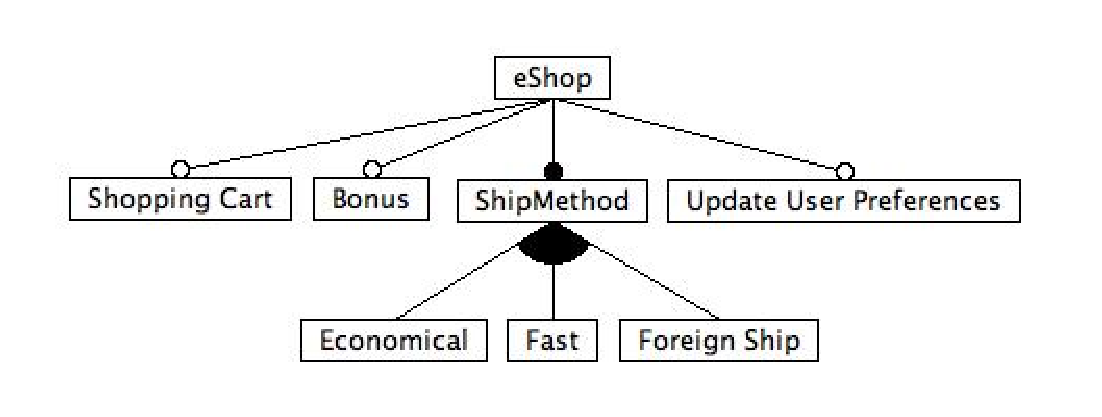
\includegraphics[scale=0.40]{../images/eShop-fm-re.eps}
   \caption{Subset of eShop feature model.}
  \label{fig:eshop-fm-re}
  \end{center}
\end{figure}

Notice that \emph{Proceed to Purchase} and \emph{Search for Products} scenarios
are mandatory (Table~\ref{tab:ck-running-example}), since they are related to a feature
expression that allways hold \emph{true} (the root feature). Other scenarios
will be present only if the related expression is evaluated as \emph{true} for
the specific product being generated.

\begin{table}[bth]
\begin{center}
 \caption{eShop configuration knowledge}
\label{tab:ck-running-example}
\begin{tabular}{ll}
   \hline\noalign{\smallskip}
  {\bf Expression} & {\bf Required Scenarios} \\
   \noalign{\smallskip}
   \hline
   \noalign{\smallskip}
    eShop & Proceed to Purchase \\
               & Search for Products \\
               & \ldots \\ 
    {\bf not} (Cart {\bf and} Bonus)\hspace{2pt} & Buy a Product \\ 
    Cart {\bf and} Bonus & Buy Products with Cart \\ 
    Update Preferences & Register User Preferences	 \\  
    \ldots & \ldots \\ 
  \hline
\end{tabular}
\end{center}
\end{table}

Listing~\ref{lst:configure} presents the product derivation function
(\emph{pdWeaver}), which corresponds to the reference implementation for
the \emph{optional use cases and scenarios} technique. This function takes as
input a \emph{SPL use case model} (UCM), a \emph{feature model} (FM), a \emph{product
configuration} (PC), and a \emph{configuration knowledge} (CK).

Initially, this function verifies if the product configuration is a well formed
instance of the feature model (Line 3 in Listing~\ref{lst:configure}) --- if it is not
the case,  an \emph{InvalidProduct} error is thrown. Then, the IDs of selected
scenarios are filtered by the \emph{configure} function. This is done by
evaluating which feature expressions, defined in the list elements (\emph{x:xs})
of the configuration knowledge, are valid for the specific product instance
(\emph{eval} function). Finally, given the resulting list of scenario IDs, the function
\emph{retrieveScenarios} returns the product specific scenarios. 

\begin{lstlisting}[belowskip=10pt,frame=tb,caption={Product derivation weaver function},label=lst:configure]
pdWeaver :: UCM -> FM -> PC -> CK -> ScenarioList
pdWeaver ucm fm pc ck = 
 if not (validInstance fm pc) 
  then error InvalidProduct
  else retrieveScenarios ucm (configure pc ck)

configure :: PC -> CK -> ListOfScenarioId
configure pc (CK []) = []
configure pc (CK (x:xs)) =
 if (eval pc (expression x))
  then (artifacts x) ++ (configure pc (CK xs))
  else configure pc (CK xs)
\end{lstlisting} 

It is important to notice that this variation technique presents two levels of
crosscutting. First, the feature model, the product configuration, and
the configuration knowledge crosscut each other with respect to the
list of valid scenario IDs. Then, the resulting list of scenario IDs crosscuts
with the use case model for selecting the product specific scenarios.   

The model of the \emph{optional use cases and scenarios} technique, in terms of
our modeling framework, is shown in Table~\ref{tab:pd-weaver}. The
\emph{pdWeaver} function is used to argue that the model is realizable and
appropriate. We achieve this by matching the model elements to corresponding
parameters and auxiliary functions in the reference implementation. Therefore,
the input models UCM, FM, CK, and PC are represented as different parameters of
the \emph{pdWeaver} function. An instance of the UCM corresponds to the
specification of all SPL scenarios. A FM instance is only responsible for
declaring the SPL features and the relationships between them. As a consequence,
there is no coupling between FMs and UCMs. On the other hand, relationships
between features and artifacts are documented in the configuration knowledge. Finally, the PC
specifies which features were selected for a specific product. We present a
discussion about coupling in Section~\ref{sec:evaluation}.


The UCM has a greater importance over the other input languages ($UCM_{EFF}$),
since it declares the product specific scenarios (the output of this weaver
process generated by the \emph{pdWeaver} function). These scenarios ($UCM_{ID}$) are used
in the \emph{retrieveScenarios} function in order to identify which artifacts
will be assembled in the final product.

In order to identify which artifacts are required for a specific product, the
\emph{configure} function ($CK_{EFF}$) checks the feature expression ($CK_{ID}$)
against the product specific features ($PC_{ID}$). The effect of FM in this
weaver ($FM_{EFF}$) is to check if the PC is well formed. Such evaluation is
implemented by the \emph{validInstance} function and considers the PC feature
selection ($PC_{EFF}$). 

\begin{table}[htb]
\begin{center}
 \caption{Model of Product Derivation} \label{tab:pd-weaver}
\begin{tabular}{p{0.6in}p{2.4in}}
   \hline\noalign{\smallskip}
  {\bf Element} & {\bf Description} \\
   \noalign{\smallskip}
   \hline
   \noalign{\smallskip}
   $o$               & Product specific scenarios (list of scenarios) \\ 
   $o_{jp}$        & Scenario declarations \\ 
   $L$               & \{UCM, FM, CK, PC\} \\ 
   $UCM_{ID}$ & SPL scenarios \\ 
   $FM_{ID}$    & SPL features \\ 
   $CK_{ID}$    & Feature expressions and scenario IDs\\  
   $PC_{ID}$    & Product specific feature selection \\ 
   $UCM_{EFF}$ & Provides declaration of scenarios \\  
   $FM_{EFF}$    & Checks if a SPL instance is well formed \\ 
   $CK_{EFF}$    & Identifies selected artifacts  \\ 
   $PC_{EFF}$    &Triggers scenario selection \\
   $UCM_{MOD}$ & Scenario \\  
   $FM_{MOD}$   & Feature \\ 
   $CK_{MOD}$    & Each pair $(expression, artifact\ list)$  \\ 
   $PC_{MOD}$    & Feature \\
  \hline
  \end{tabular}
\end{center}
\end{table}

As mentioned before, it is beyound the scope of this paper presenting other
instances of our modeling framework, although we have already instantiated it
for two other scenario variability techniques: \emph{quantified changed
scenarios} and \emph{parameterized scenarios}. Next, we point some activities
that we have planed to evolve our variability model.

\subsection{Modeling framework improvements}

Previous results of our work reveal to us research activities that can
be conduced in the scope of our modeling framework. Below we summarize part of
these activities.

\begin{description}
  \item [Improve type checking] The current version of our variability
  framework is structured in a single phase, responsible for both type checking and
  for weaving the input models. Recently, we have realized the importance of
  checking properties of the input models before the composition process.
  These properties correspond to \emph{pre-conditions} that should hold, in
  order to verify the correctness of a composition. Therefore, this activity
  aims to identify other properties that should be checked and reestructure our
  variability framwork to modularize type checking and composition processes in
  different phases.
  \item [Improve the configuration knowledge] The variability techniques that
  we have represented~\cite{} are well supported by a model of
  configuration knowledge that relates feature
  expressions to artifacts. If a feature expression is valid for a
  specific instance, the related artifacts will be assembled in the final
  product. However, we have identified other kinds of scenario variability that
  can be easly represented using a more expressive view of the configuration
  knowledge. In this view, feature expressions are related to \emph{model
  transformations}, instead of being related to software artifacts. If a
  feature expression is valid for a specific instance, the \emph{model
  transformation} will be applied. However, we have not evaluated this design
  yet.
  \item [Apply our model to other contexts] Until now, we have applied our
  variability framework for the context of use case scenarios. As a future
  work, we aim at representing, using our approach, techniques for SPL test
  case variability. By doing that, we will be able to identify, more
  precisaly, the real benefits regarded to SPL traceability.
\end{description}
 
The next section presents some results that we have achieved based on
evaluating our approach. Additionally, it also presents future activities for
improving the evaluation process.

% -------------------------------------------------------------------------
\section{Evaluation}\label{sec:evaluation}

In a previous paper~\cite{Bonifacio:2008aa}, we reported on the benefits of a
clear separation between variability management and use case scenarios. We
achieved such a result by comparing our approach with
PLUC~\cite{Bertolino:2003aa} and PLUSS~\cite{Eriksson:2005aa}, two representative notations for SPL scenario
variability. In order to increase our confidence, different techniques for
evaluating modularity had been used: \emph{Design Structure Matrices} 
(Section~\ref{sub:dsm})), quantitative analysis associated to a proposed
metric suite (Section~\ref{sub:metrics}), and observations of the
effort needed to introduce SPL increments using each approach (Section~\ref{sub:increments}).

In this section, we are going to present just the evaluation techniques.
Detailed results of our analysis can be found
elsewhere~\cite{Bonifacio:2008aa,Bonifacio:2008ab}. Additionally,
Section~\ref{sub:eval-improvments} presents how we are planning to evolve our evaluation
process.

\subsection{Design Structure Matrices (DSMs)}\label{sub:dsm}

DSMs is an interesting and simple tool for visualizing dependencies between
design decisions~\cite{Baldwin:2000aa}. Such decisions appear in the rows and
columns of a matrix. We can identify a dependency by observing the columns in a
given row~\cite{Baldwin:2000aa}. For example, the first row in
Figure~\ref{dsm:pluc} indicates that design decisions regarded to variability
space (feature model) depends on the task of creating the use case models in the
PLUC approach~\cite{Bertolino:2003aa}. The first can not be independently
performed after the second. This occurs because variability space is specified at
specific sections of use cases scenarios in PLUC. Therefore, it is not possible
to evolve variability management (introducing new features, products, or
relations between features and artifacts) without reviewing the use case model.
This is expressed in the non modular DSM of Figure~\ref{dsm:pluc}, which depicts
cyclical dependencies between use cases and variability management artifacts.

\begin{figure}[htb]
\centering
\begin{small}
\begin{tabular}{llllll} \hline
&  & 1 & 2 & 3 & 4 \\ \hline
1 & Feature model 			& 	& x	& 	&   	\\ 
2 & Use case model 		& x 	&  	&  x	&  x  \\ 
3 & Product configurations	& x 	& x	& 	&    	\\
4 & Configuration knowledge 	& x 	& x 	& 	&    	\\ \hline
\end{tabular}
\end{small}
 \caption{DSM Analysis of PLUC}
\label{dsm:pluc}
\end{figure}

Our approach reduces the dependencies between variability management and scenario
specifications (Figure~\ref{dsm:cc}). For instance, changes in feature model or
new definitions of products do not require changes in the use case model. This
clear separation is also desirable in source code, as claimed
in~\cite{Alves:2006aa, Apel:2006aa}, and might be required in other artifacts
too. 

\begin{figure}[h]
\centering
\begin{small}
\begin{tabular}{lllllll} \hline
& & 1 & 2 & 3 & 4 & 5 \\ \hline
1 & Feature model 		& 	& 	&      &  	&  	\\ 
2 & Mapping	 		& x	&	&	&	&  	\\
3 & Use case model 	&  	&  x	&  	&  	& 	\\
4 & SPL instances 		& x 	& 	& 	&   	& 	\\
5 & Configuration model 	& x 	&  	&  x	&  	& 	\\  \hline
\end{tabular}
\end{small}
 \caption{DSM Analysis of our approach}
\label{dsm:cc}
\end{figure}   

We have applyed DSMs to visualize design dependencies in two levels: the first
one presents a high level view of dependencies between variability management
(feature model, SPL instances and configuration model) and use cases (as shown in
Figure~\ref{dsm:pluc} and Figure~\ref{dsm:cc}); the second one presents how
features are spread among use cases. Although we do not present any example of
the second level of DSM in this paper, it is very useful for computing several
of the metrics present in the next section.


\subsection{Proposed metric suite}\label{sub:metrics}

We derived several metrics for quantifying feature modularity and use case model
complexity (related to the size of specifications)~\cite{Bonifacio:2008aa}.
Increasing levels of feature modularity implies better evolv- ability, since SPL
changes or increments can be performed in a isolated way. Also, if a modular
feature specification could crosscut other specifications, it would be expected
more reusable assets. The metric suite described in this section was adapted
from~\cite{Garcia:2005aa} for both product line and use cases contexts. It quantifies 
feature modularity and use case complexity. 

The proposed modularity metrics quantify three types of relations involving
features and use cases. First, \emph{Feature Diffusion over Use Cases} (FDU) is
used for quantifying how many use cases are affected by a specific feature. On
the other hand, \emph{Number of Features per Use Case} (NFU) is used for
quantifying how many features are tangled within a specific use case. We assume
that each use case should focus on its primary goal, although several features
might be related to the primary goal of a use case. Finally, we applied the
metric \emph{Feature Diffusion over Scenarios} (FDS) in order to quantify how
many internal use case members (scenarios) are necessary for the materialization
of a specific feature.
 
Additionally, we used three metrics related to complexity. The first one,
\emph{Vocabulary Size}, quantifies the number of use cases (VSU) and scenarios
(VSS) required by each of the evaluated approaches. The second one, \emph{Steps
of Specification} (SS), is related to the size of each scenario and identifies
how many pairs \emph{User action} x \emph{System response} compose a specific
scenario. Additionally, we also relate modularity to complexity by applying
\emph{Features and Steps of Specification} (FSS), which counts the number of
steps of specification whose main purpose is to describe the behavior of a
feature. A complete description of these metrics can be found
elsewhere~\cite{Bonifacio:2008aa}.

Table~\ref{tab:metrics} summarizes the evaluation of these metrics applied to
one of our case studies --- a real multimedia message (MMS) product
line~\cite{Bonifacio:2008aa}. Next, we present the third kind of evalation,
which tryies to quantify SPL evolvability by observing the impact of introducing
common SPL changes.

\begin{table}[htb]
\centering
\caption{Modularity and complexity metrics}
\label{tab:metrics}
\begin{small}
\begin{tabular}{lccc} \hline
					    & PLUC 	& PLUSS 	& Crosscutting	\\ \hline
Mean value of FDU 		& 3.5	& 3.5	& 2					\\
Mean value of FDS 		& 6.25	& 5		& 4.25				\\
Mean value of NFU 		& 2		& 2		& 1					\\
Mean value of FSS 		& 12	& 11	& 10.25				\\ 
VSU 					& 5		& 5		& 7					\\
VSS 					& 27	& 24	& 23				\\
SS 					    & 75	& 64	& 56				\\	\hline
\end{tabular}
\end{small}
\end{table}

\subsection{SPL evolution analysis}\label{sub:increments}

Besides applying DSM analysis and
quantitative analysis, we also evaluated the impact needed to introduce a few
increments in the MMS product line, whose original version was specified in the
three evaluated approaches~\cite{Bonifacio:2008aa}. 

In this evaluation, we basicaly proposed three scenarios of changing that were
suppose to occur in the MMS product line. The new version of MMS product line 
introduced a new \emph{structured data operation}, allowing a subscriber to make
a call for a number embedded in a message; introduced a new
\emph{content type}, allowing a subscriber to attach emotion icons
to messages; and defined new product instances. These scenarios of modification
were signifficant because the first one required changes in the behavior,
the second one required changes in scenario parameters, and the last one
required changes in the variability models. 

The conclusion of this evaluation enforce that a clear separation of
variability management and scenario specifications, as supported by PLUSS and by
our approach, is necessary to improve SPL evolvability. However, in order to
enhance our confidence, more controlled studies should be performed in this
thesis. In what follows, we present possible improvements in our evaluation
process. 

\subsection{Evaluation improvements}\label{sub:eval-improvments}

Although we have performed some empirical studies using our approach, and
compared it with existing ones, the level of control in these studies can be
considered low. Therefore, performing a formal experiment is the primary
improvement of our evaliation process. The goal of this experiment is twofold:
confirm the benefits of a clear separation between variablity models and use
case scenarios; and validate (or enhance) our proposed metric suite. Due to
space constraints, we just present an overview of our initial experiment design.

The experiment will be conduced as a class activity, involving undergraduate
Computer Science students. They will be responsible for specifying and evolving
scenarios of different SPLs. The technique used for specifying scenarios will be
used as the treatment variable of our experiment~\cite{Pfleeger:1994aa}.
Dependend on the number of techniques that will be evaluated, two or three
systems are going to be specified. Therefore, if just PLUSS and our approach are
going to be compared, just two SPLs will be used in our experiment. On the other
hand,if PLUC, PLUSS, and our approach are going to be compared, three SPLs
will be used.

Students and SPLs are the two variables (or factors) that must be controled. In
order to minimize the \emph{experimental error} motivated by such
variables~\cite{Pfleeger:1994aa}, we have to randomize the activities in such a
way that each student will be assigned to each evaluated technique and SPL. An
interesting layout for this initial arrangement is the \emph{Latin Square}
design~\cite{Box:2004aa}. The response variables will be the time needed to
specify the SPLs and to perform a sequence of changes.

% -------------------------------------------------------------------------
\section{Related work}\label{sec:related}


{\bf Scenario Variability.} Several approaches have been proposed for
representing scenario variability~\cite{Jacobson:1997aa, Griss:1998aa,
Eriksson:2005aa,Bertolino:2003aa}. However, in this work we only compare our
crosscutting approach with PLUC and PLUSS techniques because they encompass a
broad range of SoC between variability management and scenario specification.
Moreover, they were propose specifically for representing variability in SPLs. It
is important to notice that the primary goal of existing approaches is to provide
variation points in use case scenarios. Hence, the main contribution of our
crosscutting approach is that we introduce the perspective of creating a better
separation between variability management and scenario specification.
 
{\bf Modularity Assestment.} Design Structure Matrices (DSMs) and crosscutting
metrics have been applied for assessing modularity in \emph{aspect-oriented}}
systems~\cite{Lopes:2005ab,Sullivan:2005aa, Garcia:2005aa, Greenwood:2007aa,
Figueiredo:2008aa}. In this work, we also applied DSMs in the context of scenario variability management. Moreover, we
customized a suite of metrics for quantifying feature diffusion and tangling over
use cases. To our knowledge, our work is unique in applying both DSMs and
crosscutting metrics for evaluating SoC in scenario variability.


\section{Concluding remarks}\label{sec:concludings}

% Apresentar uma visao geral
% DISCUTIR SOBRE O SUPORTE FERRAMENTAL
% Resumir as atividades futuras
%------------------------------------------------------------------------- 

\bibliographystyle{latex8}
\bibliography{../references/phd-references}

\end{document}

